\documentclass[a4paper,11pt]{report}
\usepackage[showexo=true,showcorr=false,showdegree=true]{../packages/coursclassed}
%Commenter ou enlever le commentaire sur la ligne suivante pour montrer le niveau
\toggletrue{montrerNiveaux}
%permet de gérer l'espacement entre les items des env enumerate et enumitem
\usepackage{enumitem}
\setlist[enumerate]{align=left,leftmargin=1cm,itemsep=10pt,parsep=0pt,topsep=0pt,rightmargin=0.5cm}
\setlist[itemize]{align=left,labelsep=1em,leftmargin=*,itemsep=0pt,parsep=0pt,topsep=0pt,rightmargin=0cm}
%permet de gerer l'espacement entre les colonnes de multicols
\setlength\columnsep{35pt}

\usepackage{numprint}

\begin{document}

%%%%%%%%%%%%%%%%% À MODIFIER POUR CHAQUE SERIE %%%%%%%%%%%%%%%%%%%%%%%%%%%%%
\newcommand{\chapterName}{Fonctions et algèbre}
\newcommand{\serieName}{Proportionnalité : Les pourcentages}

%%%%%%%%%%%%%%%%%% PREMIERE PAGE NE PAS MODIFER %%%%%%%%%%%%%%%%%%%%%%%%
% le chapitre en cours, ne pas changer au cours d'une série
\chapter*{\chapterName}
\thispagestyle{empty}

%%%%% LISTE AIDE MEMOIRE %%%%%%
\begin{amL}{\serieName}{
\item Proportionnalité - Généralités (page 55)
\item Résoudre un problème de proportionnalité (page 57)
\item Pourcentage (page 58)
\item Déterminer un pourcentage (page 58)
}\end{amL}

%%%%%%%%%%%%%%% DEBUT DE LA SERIE NE PAS MODIFIER %%%%%%%%%%%%%%%%%%%%%%%%%%%%%
\section*{\serieName}
\setcounter{page}{1}

%%%%%%%%%%% LES EXERCICES %%%%%%%%%%%%%%%%%%%%%%%%%%%%%%%%%%%%





% Fraction - Nombre décimal - Pourcentage

\begin{exop}{
Complète.
\begin{tasks}(2)
    \task $\dfrac{1}{4}=\dfrac{}{100}$
    \task $\dfrac{10}{100}=\dfrac{1}{}$
    \task $\dfrac{75}{100}=\dfrac{}{4}$
    \task $\dfrac{}{100}=\dfrac{1}{5}$
    \task $\dfrac{1}{2}=\dfrac{50}{}$
    \task $\dfrac{1}{}=\dfrac{5}{100}$
\end{tasks}
}{1}    
\end{exop}

\begin{exop}{
Complète.
\begin{tasks}(2)
    \task $\dfrac{2}{}=\dfrac{40}{100}$
    \task $\dfrac{60}{}=\dfrac{3}{5}$
    \task $\dfrac{3}{10}=\dfrac{30}{}$
    \task $\dfrac{}{100}=\dfrac{11}{5}$
    \task $\dfrac{1}{20}=\dfrac{5}{}$
    \task $\dfrac{14}{}=\dfrac{7}{50}$
\end{tasks}
}{1}    
\end{exop}


\begin{exof}{FA63}{90}{1} % nb décimal - %
\end{exof}

%%%%%%%%%%%%%%%
%%%%%%%%%%%%%%%
%%%%%%%%%%%%%%%
%%%%%%%%%%%%%%%
%%%%%%%%%%%%%%% STP NATHAN PEUX-TU AMELIORER LA PRESENTATION DE CET EXERCICE RESOLU ? J'IMAGINE AJOUTER DES PETITES FLECHES POUR INDIQUER LE FACTEUR DE PROPORTIONNALITE
%%%%%%%%%%%%%%%
%%%%%%%%%%%%%%%
%%%%%%%%%%%%%%%
%%%%%%%%%%%%%%%

\begin{resolu}{Calculer une partie d'un tout}{
    Calcule.
    \begin{tasks}(1)
    \task $10\%$ de \tunit{95}{CHF} = \hrulefill %\underline{$10\%\cdot95=\frac{10}{100}\cdot95=9,5=\tunit{9,50}{CHF}$}

     \begin{minipage}[]{0.3\textwidth}
     \begin{tabular}{|c|c|c|}
         \hline
         partie & $10$ & \\ \hline
         tout & $100$ & $95$ \\ \hline
     \end{tabular}
     \end{minipage}
     \begin{minipage}[]{0.8\textwidth}
        Facteur de prop. : $\dfrac{10}{100}=0,1$
        
        $95\cdot0,1=\tunit{9,50}{CHF}$
     \end{minipage}

    \task $30\%$ de \tunit{360}{CHF} = \hrulefill %\underline{$30\%\cdot360=\frac{30}{100}\cdot360=\tunit{108}{CHF}$}

    \begin{minipage}[]{0.3\textwidth}
     \begin{tabular}{|c|c|c|}
         \hline
         partie & $30$ & \\ \hline
         tout & $100$ & $360$ \\ \hline
     \end{tabular}
     \end{minipage}
     \begin{minipage}[]{0.7\textwidth}
        Facteur de prop. : $\dfrac{30}{100}=0,3$
        
        $360\cdot0,3=\tunit{108}{CHF}$
     \end{minipage}
     
    \task $50\%$ de \tunit{70}{CHF} = \hrulefill %\underline{$50\%\cdot70=\frac{50}{100}\cdot70=\tunit{35}{CHF}$}

    \begin{minipage}[]{0.3\textwidth}
     \begin{tabular}{|c|c|c|}
         \hline
         partie & $50$ & \\ \hline
         tout & $100$ & $70$ \\ \hline
     \end{tabular}
     \end{minipage}
     \begin{minipage}[]{0.7\textwidth}
        Facteur de prop. : $\dfrac{50}{100}=0,5$
        
        $70\cdot0,5=\tunit{35}{CHF}$
     \end{minipage}
     
    \task $75\%$ de \tunit{40}{CHF} = \hrulefill %\underline{$75\%\cdot40=\frac{75}{100}\cdot40=\tunit{30}{CHF}$}

    \begin{minipage}[]{0.3\textwidth}
     \begin{tabular}{|c|c|c|}
         \hline
         partie & $75$ & \\ \hline
         tout & $100$ & $40$ \\ \hline
     \end{tabular}
     \end{minipage}
     \begin{minipage}[]{0.7\textwidth}
     Facteur de prop. : $\dfrac{75}{100}=0,75$
        
        $40\cdot0,75=\tunit{30}{CHF}$
     \end{minipage}
\end{tasks}
}{1}    
\end{resolu}

\begin{exop}{
Calcule.
\begin{tasks}(1)
    \task $10\%$ de \tunit{40}{CHF} = \hrulefill
    \task $20\%$ de \tunit{40}{CHF} = \hrulefill
    \task $40\%$ de \tunit{40}{CHF} = \hrulefill
    \task $70\%$ de \tunit{40}{CHF} = \hrulefill
\end{tasks}
}{1}    
\end{exop}

\begin{exop}{
Calcule.
\begin{tasks}(1)
    \task $10\%$ de \tunit{60}{CHF} = \hrulefill
    \task $30\%$ de \tunit{60}{CHF} = \hrulefill
    \task $70\%$ de \tunit{60}{CHF} = \hrulefill
    \task $150\%$ de \tunit{60}{CHF} = \hrulefill
\end{tasks}
}{1}    
\end{exop}



\begin{exop}{
    Calcule.
    \begin{tasks}
        \task les $10\%$ de \tunit{150}{CHF} = \hrulefill
        \task les $25\%$ de \tunit{280}{m} = \hrulefill
        \task les $50\%$ de \tunit{400}{cm^3} = \hrulefill
        \task les $75\%$ de \tunit{240}{litres} = \hrulefill
        \task les $10\%$ de \tunit{450}{m^3} = \hrulefill
        \task les $50\%$ de \tunit{50}{CHF} = \hrulefill
    \end{tasks}
}{1}
\end{exop}


\begin{exop}{
Calcule.
\begin{tasks}(1)
    \task les $4,5\%$ de \tunit{750}{CHF} = \hrulefill
    \task les $26\%$ de \tunit{2700}{CHF} = \hrulefill
    \task les $3,5\%$ de \tunit{8250}{kg} = \hrulefill
    \task les $28\%$ de \tunit{325}{m} = \hrulefill
\end{tasks}
}{1}    
\end{exop}

\begin{exop}{
Calcule.
\begin{tasks}(1)
    \task les $73\%$ de \tunit{4200}{personnes} = \hrulefill
    \task les $15\%$ de \tunit{47,40}{CHF} = \hrulefill
    \task les $68\%$ de \tunit{4570}{kg} = \hrulefill
    \task les $29\%$ de $\numprint{42580000}$ personnes = \hrulefill
\end{tasks}
}{1}    
\end{exop}


\begin{resolu}{Calculer un pourcentage}{
    Complète.
    \begin{tasks}(1)
    \task Les $\ligne{2}\%$ de \tunit{95}{CHF} = \tunit{9,50}{CHF}

    \begin{minipage}[]{0.3\textwidth}
     \begin{tabular}{|c|c|c|}
         \hline
         partie &  & $9,5$ \\ \hline
         tout & $100$ & $95$ \\ \hline
     \end{tabular}
     \end{minipage}
     \begin{minipage}[]{0.7\textwidth}
        Facteur de prop. : $\dfrac{9,5}{95}=0,1$
        
        $100\cdot0,1=\tunit{10}{\%}$
     \end{minipage}
    
    \task Les $\ligne{2}\%$ de \tunit{360}{CHF} = \tunit{108}{CHF}
    
    \begin{minipage}[]{0.3\textwidth}
     \begin{tabular}{|c|c|c|}
         \hline
         partie &  & $108$ \\ \hline
         tout & $100$ & $360$ \\ \hline
     \end{tabular}
     \end{minipage}
     \begin{minipage}[]{0.7\textwidth}
     Facteur de prop. : $\dfrac{108}{360}=0,3$
     
        $100\cdot0,3=\tunit{30}{\%}$
     \end{minipage}
    
    \task Les $\ligne{2}\%$ de \tunit{70}{CHF} = \tunit{35}{CHF} 

    \begin{minipage}[]{0.3\textwidth}
     \begin{tabular}{|c|c|c|}
         \hline
         partie &  & $35$ \\ \hline
         tout & $100$ & $70$ \\ \hline
     \end{tabular}
     \end{minipage}
     \begin{minipage}[]{0.7\textwidth}
     Facteur de prop. : $\dfrac{35}{70}=0,5$
     
        $100\cdot0,5=\tunit{50}{\%}$
     \end{minipage}
    
    \task Les $\ligne{2}\%$ de \tunit{40}{CHF} = \tunit{30}{CHF}
    
    \begin{minipage}[]{0.3\textwidth}
     \begin{tabular}{|c|c|c|}
         \hline
         partie &  & $30$ \\ \hline
         tout & $100$ & $40$ \\ \hline
     \end{tabular}
     \end{minipage}
     \begin{minipage}[]{0.7\textwidth}
     Facteur de prop. : $\dfrac{30}{40}=0,75$
     
        $100\cdot0,75=\tunit{75}{\%}$
     \end{minipage}
    
\end{tasks}
}{1}    
\end{resolu}

\begin{exo}{
    Complète.
    \begin{tasks}
        \task les \ligne{2}$\%$ de \tunit{350}{m} = \tunit{35}{m}
        \task les \ligne{2}$\%$ de \tunit{180}{litres} = \tunit{90}{litres}
        \task les \ligne{2}$\%$ de \tunit{240}{cm^3} = \tunit{60}{cm^3}
        \task les \ligne{2}$\%$ de \tunit{80}{CHF} = \tunit{60}{CHF}
        \task les \ligne{2}$\%$ de \tunit{76}{m^3} = \tunit{38}{m^3}
        \task les \ligne{2}$\%$ de \tunit{120}{CHF} = \tunit{12}{CHF}
    \end{tasks}
}{1}    
\end{exo}


\begin{exo}{
    Complète.
    \begin{tasks}
        \task les \ligne{2}$\%$ de \tunit{150}{CHF} = \tunit{45}{CHF} %30
        \task les \ligne{2}$\%$ de \tunit{270}{m} = \tunit{27}{m} %10
        \task les \ligne{2}$\%$ de \tunit{60}{cm^3} = \tunit{9}{cm^3} %15
        \task les \ligne{2}$\%$ de \tunit{200}{litres} = \tunit{40}{litres} %20
        \task les \ligne{2}$\%$ de \tunit{350}{m^3} = \tunit{280}{m^3} %80
        \task les \ligne{2}$\%$ de \tunit{120}{CHF} = \tunit{60}{CHF} %50
    \end{tasks}
}{1}    
\end{exo}



\begin{resolu}{Calculer le tout d'une partie}{
    Calcule.
    \begin{tasks}(1)
    \task $10\%$ de \ligne{2} = \tunit{9,50}{CHF}
    
        \begin{minipage}[]{0.3\textwidth}
         \begin{tabular}{|c|c|c|}
             \hline
             partie & $10$ & $9,50$ \\ \hline
             tout & $100$ &  \\ \hline
         \end{tabular}
         \end{minipage}
         \begin{minipage}[]{0.7\textwidth}
         Facteur de prop. : $\dfrac{10}{100}=0,1$
         
            $9,50 : 0,1 =\tunit{95}{CHF}$
         \end{minipage}
     
    \task $30\%$ de \ligne{2} = \tunit{108}{CHF}
    
        \begin{minipage}[]{0.3\textwidth}
         \begin{tabular}{|c|c|c|}
             \hline
             partie & $30$ & $108$ \\ \hline
             tout & $100$ &  \\ \hline
         \end{tabular}
         \end{minipage}
         \begin{minipage}[]{0.7\textwidth}
         Facteur de prop. : $\dfrac{30}{100}=0,3$
         
            $108 : 0,3=\tunit{360}{CHF}$
         \end{minipage}
     
    \task $50\%$ de \ligne{2} = \tunit{35}{CHF}
    
        \begin{minipage}[]{0.3\textwidth}
         \begin{tabular}{|c|c|c|}
             \hline
             partie & $50$ & $35$ \\ \hline
             tout & $100$ &  \\ \hline
         \end{tabular}
         \end{minipage}
         \begin{minipage}[]{0.7\textwidth}
         Facteur de prop. : $\dfrac{50}{100}=0,5$
         
            $35 : 0,5=\tunit{70}{CHF}$
         \end{minipage}
     
    \task $75\%$ de \ligne{2} = \tunit{30}{CHF}
    
        \begin{minipage}[]{0.3\textwidth}
         \begin{tabular}{|c|c|c|}
             \hline
             partie & $75$ & $30$ \\ \hline
             tout & $100$ &  \\ \hline
         \end{tabular}
         \end{minipage}
         \begin{minipage}[]{0.7\textwidth}
         Facteur de prop. : $\dfrac{75}{100}=0,75$
         
            $30 : 0,75=\tunit{40}{CHF}$
         \end{minipage}
     
\end{tasks}
}{1}    
\end{resolu}




\begin{exof}{FA64}{90}{1} % calcul 
\end{exof}

\begin{resolu}{Trouver un pourcentage par complétion}{
    Joëlle et Vanessa se partagent une pizza. Joëlle en mange les $55\%$. Quel pourcentage de pizza reste-t-il pour Vanessa ?
    \begin{multicols}{2}
    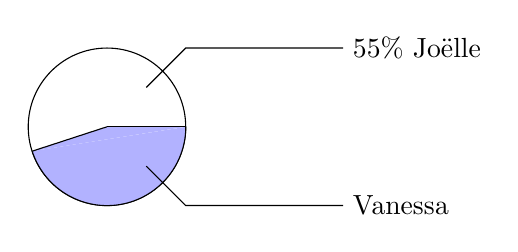
\begin{tikzpicture}
        \draw (0,0) circle (1) ;
        %\draw[fill=blue!30]  (1,0) arc (0:198:1) ;
        \draw[fill=blue!30]  (-0.95,-0.31) arc (198:360:1) ;
        \fill[color=blue!30] (-0.95,-0.31) -- (1,0) -- (0,0) -- cycle ;
        %\draw[fill=red]  (-1,0) arc (180:198:1) ;
        \draw (0,0) -- (1,0) ;
        \draw (0,0) -- (-0.95,-0.31) ;
        \draw (0.5,0.5) -- (1,1) -- (3,1) ;
        \node[anchor=west] at (3,1) {$55\%$ Joëlle} ;
        \draw (0.5,-0.5) -- (1,-1) -- (3,-1) ;
        \node[anchor=west] at (3,-1) {Vanessa} ;
    \end{tikzpicture}
    
    On sait que la totalité de la pizza correspond à $100\%$.
    
    Il reste donc $100\%-55\%=45\%$ de pizza pour Vanessa.
    \end{multicols}
}{1}
\end{resolu}


\begin{exop}{
À la surface de notre planète, il y a $71\%$ de mers et d'océans. Quel est le pourcentage des terres ?

Réponse : \hrulefill
}{1}    
\end{exop}


\begin{exop}{
Trois frères se partagent un bénéfice en fonction de leur implication dans l'entreprise. Le premier reçoit $30\%$ du bénéfice. Le deuxième en reçoit $25\%$. Quel pourcentage du bénéfice recevra le troisième frère ?

Réponse : \hrulefill
}{1}    
\end{exop}

\begin{exop}{
Lissandro a obtenu $87\%$ de réponses justes à son examen. Quel est le pourcentage de réponses erronées ?

Réponse : \hrulefill
}{1}    
\end{exop}


\begin{exop}{
Une méthode de gestion budgétaire propose de répartir ses revenus de la manière suivante :
\begin{itemize}
    \item $50 \%$ consacrés aux dépenses essentielles (logement, nourriture, transports, assurances, etc.).
    \item $30 \%$ dédiés aux dépenses personnelles et aux loisirs.
    \item Le reste est réservé à l'épargne et aux investissements.
\end{itemize}

Quel pourcentage est réservé à l'épargne et aux investissements ?

Réponse : \hrulefill
}{1}    
\end{exop}


% A) Trouver le montant d'une réduction/augmentation

\begin{exo}{
Une pièce de tissu mesure \tunit{120}{m}. On en vend les $42\%$.

Quelle longueur (en m) reste-t-il ?
}{1}    
\end{exo}

\begin{exo}{
Aristote désire acheter un radio-réveil à \tunit{185}{CHF}. Le magasin accorde un rabais de $10\%$. A combien s'élève le rabais et quel sera le prix payé pour ce radio-réveil ?
}{1}
\end{exo}

\begin{exo}{
Sakura achète un vélo \tunit{220}{CHF}. Elle le répare et le revend en faisant un bénéfice de $30\%$.
Quel est le montant du bénéfice réalisé ? Quel est le prix de vente ?
}{1}
\end{exo}

\begin{exo}{
Dans une école de $250$ élèves, on a procédé à une élection. $250$ bulletins de vote ont été distribués. 

Trois élèves se présentaient pour le poste de délégué.

\begin{itemize}
    \item Talia a obtenu $32\%$ des voix ;
    \item Mia a obtenu $40\%$ des voix ;
    \item Christopher a obtenu $20\%$ des voix ;
    \item $8\%$ des bulletins étaient nuls.
\end{itemize}

Combien de voix a obtenu chaque élève ?
}{1}    
\end{exo}

\begin{exo}{
La teneur en eau des pommes de terre est de $78\%$, celle des noix est de $5\%$ et celle des oignons blancs de $60\%$.
\begin{tasks}(1)
    \task Quelle est la quantité d'eau contenue dans \tunit{3}{kg} de pommes de terre ? Dans \tunit{4,5}{kg} de pommes de terre ?
    \task Quelle est la quantité d'eau contenue dans \tunit{500}{g} de noix ? Dans \tunit{100}{g} de noix ?
    \task Quelle est la quantité d'eau contenue dans \tunit{750}{g} d'oignons blancs ? Dans \tunit{1}{kg} ? Dans \tunit{1,750}{kg} ?
\end{tasks}
}{1}    
\end{exo}


\begin{exo}{
On peut admettre qu'un être humain passe en moyenne
\begin{itemize}
    \item $30\%$ de son temps à dormir,
    \item $37\%$ de son temps à travailler,
    \item $8\%$ de son temps à manger.
\end{itemize}
En un mois, quel va être le nombre d'heures consacrées respectivement au sommeil, au travail et aux repas ?
}{1}    
\end{exo}

\begin{exo}{
L'air que nous respirons contient $23\%$ d'oxygène, $76\%$ d'azote et $1\%$ de gaz rares. L'air contenu dans une pièce a une masse de \tunit{52}{kg}.

Quelle est la masse d'oxygène contenue dans la pièce ? Quelle est la masse d'azote ? Et celle de gaz rares ?
}{1}
\end{exo}

\begin{exo}{
Daisuke désire s'acheter un sac qui coûte \tunit{75}{CHF}.

Dans un premier magasin, on lui propose un rabais de $12\%$.

Dans un second magasin, on lui accorde un rabais de \tunit{8,50}{CHF}.

Dans quel magasin Daisuke va-t-il acheter son sac ?
}{1}
\end{exo}


% B) Trouver le montant de départ


\begin{exo}{
\begin{tasks}(1)
    \task Une veste coûte \tunit{150}{CHF}. Quel est le rabais en CHF si on obtient une réduction de \tunit{15}{\%} ? Finalement, quel sera le prix payé ?
    \task Le loyer du studio de Hannah est de  \tunit{1200}{CHF}. Sa régie annonce une augmentation de \tunit{8}{\%} par mois. À quel montant en CHF correspond cette augmentation ? Quel sera le montant de son nouveau loyer ?

    \task En 2023, une voiture coûtait $\numprint{23500}$ CHF. En 2024, son prix subit une augmentation de $5,5\%$. Combien coûte-t-elle aujourd'hui ?

    \task Un stylo coûte \tunit{9,50}{CHF}. Le magasin accorde une remise de $20\%$. Combien paiera-t-on ce stylo ?

    \task Zaccharia obtient un rabais de $25\%$ sur un ordinateur qui coûtait \tunit{1250}{CHF}. Quel prix va-t-il payer ?

    \task Le prix d'un litre de lait subi une baisse de $10\%$, puis une baisse de $4\%$. Calcule le prix d'un litre de lait qui coûtait initialement \tunit{3,10}{CHF}.

    \task Un sac coûte \tunit{32}{CHF} hors taxe (H.T.). Le taux de TVA est de $8\%$. Quel est le montant de la taxe ? Quel est le prix du sac toutes taxes comprises (T.T.C.) ?

    \task Juliette achète un scooter à \tunit{3550}{CHF}. À la commande, elle paie $20\%$ d'acomptes. Lorsqu'elle le reçoit, elle paie $30\%$ de ce qu'il reste à payer. Quelle somme lui reste-t-il à payer par la suite ?

    \task Un maraîcher récolte \tunit{25}{\kilo g} de tomates. Il en garde $12\%$ pour faire de la sauce tomate. Quelle masse de tomates sera utilisée pour faire de la sauce ?
\end{tasks}
}{1}    
\end{exo}

\begin{exo}{
\begin{tasks}(1)
    \task Fanta obtient un rabais de \tunit{15}{\%} sur un vélo. Calcule son prix initial si le rabais a été de \tunit{120}{CHF}.
    
    \task Mahmoud doit verser \tunit{816}{CHF} pour s'acquitter d'une facture sur laquelle un rabais de $4\%$ lui a été consenti. À combien s'élève la facture avant le rabais ?

    \task Lors des soldes, un magasin affiche $20\%$ de réduction sur tous ses articles. Yassine achète pour \tunit{180}{CHF} de vêtements.  Calcule le prix de ces vêtements avec la réduction accordée par le magasin.

    \task En 2024, une agricultrice voit sa production de cardons augmenter de $20\%$ par rapport à l'année précédente. Cette augmentation correspond à \tunit{125}{\kilo g} de cardons supplémentaires. Quelle était la masse de sa récolte en 2023 ? Et en 2024 ?
\end{tasks}
}{1}    
\end{exo}

\begin{exo}{
\begin{tasks}(1)
    \task Dans une école, $400$ élèves ont participé aux votations pour l'élection d'un nouveau délégué. Aylin a obtenu $75$ voix. Quel pourcentage de votants cela représente-t-il ?

    \task Lors d'une évaluation, j'obtiens $30$ bonnes réponses sur $40$. Quel est mon pourcentage de bonnes réponses ?

    \task Dans ma trousse, il y a $20$ stylos. $5$ d'entre eux sont bleus. Quel pourcentage de stylos bleus ai-je dans ma trousse ? Quel pourcentage de stylos qui n'écrivent pas en bleu ai-je ?

    \task Sur $650$ élèves d'une école, $380$ étudient l'allemand. $120$ élèves étudient l'italien. Le reste des élèves étudient l'anglais. Quel pourcentage des élèves étudient l'allemand ? Et l'italien ? Et l'anglais ?
    
    \task Dans un journal de $40$ pages, il y a $12$ pages de publicité. Calcule le pourcentage de pages publicitaires.

    \task Un horloger de production contrôle la qualité de $1800$ pièces. Après vérification, il constate $72$ pièces défectueuses. Quel est le pourcentage de pièces défectueuses ? Quel est le pourcentage de pièces fonctionnelles ?

    \task Une montre coûte \tunit{1250}{CHF}. Amy l'achète pour \tunit{880}{CHF}. Quel est le pourcentage de réduction appliqué par le magasin ?

    \task Sur \tunit{75}{\kilo g} d'une récolte d'ananas,  \tunit{30}{\kilo g} sont achetés par un restaurant. Quel est le pourcentage d'ananas conservés par l'agriculteur ? 
\end{tasks}
}{1}    
\end{exo}

\begin{exo}{
L'eau, en se congelant, augmente son volume de $7\%$. Combien de litres d'eau obtient-on en faisant fondre un bloc de glace de \tunit{500}{litres} ?
}{1}    
\end{exo}


\begin{exo}{
On a obtenu un rabais de $12\%$ sur une machine à laver. Calcule le prix initial si le rabais a été de :
\begin{tasks}(3)
    \task \tunit{60}{CHF}
    \task \tunit{120}{CHF}
    \task \tunit{42}{CHF}
    \task \tunit{300}{CHF}
    \task \tunit{150}{CHF}
    \task \tunit{108}{CHF}
\end{tasks}
}{1}    
\end{exo}

\begin{exo}{
On a obtenu un rabais de $15\%$ sur un article. Calcule le prix initial si le rabais a été de :
\begin{tasks}(3)
    \task \tunit{45}{CHF}
    \task \tunit{1,50}{CHF}
    \task \tunit{4,50}{CHF}
    \task \tunit{16,50}{CHF}
    \task \tunit{90}{CHF}
    \task \tunit{94,50}{CHF}
\end{tasks}
}{1}    
\end{exo}

\begin{exo}{
Une machine a fabriqué $\numprint{1500}$ pièces identiques. Le contrôle de production a éliminé les pièces défectueuses. Il y en avait :
\begin{tasks}(3)
    \task 150
    \task 60
    \task 300
    \task 600
    \task 180
    \task 75
\end{tasks}
Exprime le nombre de pièces défectueuses en pourcentage du nombre de pièces fabriquées.
}{1}    
\end{exo}
% C) Trouver le pourcentage

\begin{exo}{
Dans une épicerie, on accorde un rabais de $10\%$ sur toutes les boîtes de biscuits.
\begin{tasks}
    \task Si une boîte coûte \tunit{4,50}{CHF}, quel sera le rabais accordé ? Combien paiera-t-on cette boîte ?
    \task Quel est le prix d'une boîte si le rabais accordé est de \tunit{1,50}{CHF} ?
    \task Si on dispose de \tunit{3,50}{CHF}, quelles boîtes de biscuits peut-on choisir ?
    \begin{multicols}{2}
        A - boîte à \tunit{3,80}{CHF}

        B - boîte à \tunit{4,25}{CHF}

        C - boîte à \tunit{4}{CHF}

        D - boîte à \tunit{3,60}{CHF}
    \end{multicols}
    
\end{tasks}
}{1}    
\end{exo}


\begin{exol}{FA58}{83}{1} % trouver %
\end{exol}

\begin{exol}{FA59}{83}{1} % soldes (comparer)
\end{exol}

\begin{exol}{FA60}{83}{1} % sondage (trouver%)
\end{exol}

\begin{exol}{FA61}{83}{1} % rabais 30%
\end{exol}

\begin{exol}{FA62}{84}{1} % NHL trouver %
\end{exol}


\begin{exol}{FA65}{84}{1} % vol Sydney
\end{exol}

\begin{exol}{FA66}{85}{1} % mix
\end{exol}

\begin{exol}{FA67}{85}{1} % photocopieuse donner % d'agrandissement ou de réduction
\end{exol}

\begin{exol}{FA68}{86}{1} % réduction
\end{exol}

\begin{exol}{FA69}{86}{1} % périm-aire
\end{exol}

\begin{exol}{FA70}{86}{1} % population
\end{exol}

\begin{exol}{FA71}{86}{1} % nb élèves
\end{exol}







\end{document}
